% !TEX encoding = UTF-8 Unicode
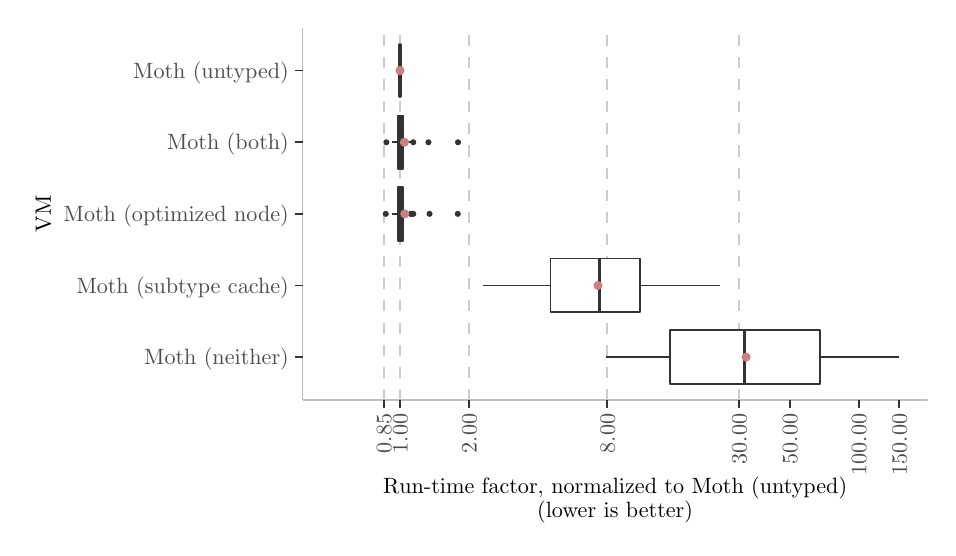
\begin{tikzpicture}[x=1pt,y=1pt]
\definecolor{fillColor}{RGB}{255,255,255}
\path[use as bounding box,fill=fillColor,fill opacity=0.00] (0,0) rectangle (325.21,180.67);
\begin{scope}
\path[clip] ( 99.31, 46.11) rectangle (325.21,180.67);
\definecolor{drawColor}{gray}{0.80}

\path[draw=drawColor,line width= 0.6pt,dash pattern=on 4pt off 4pt ,line join=round] (128.69, 46.11) -- (128.69,180.67);

\path[draw=drawColor,line width= 0.6pt,dash pattern=on 4pt off 4pt ,line join=round] (134.54, 46.11) -- (134.54,180.67);

\path[draw=drawColor,line width= 0.6pt,dash pattern=on 4pt off 4pt ,line join=round] (159.49, 46.11) -- (159.49,180.67);

\path[draw=drawColor,line width= 0.6pt,dash pattern=on 4pt off 4pt ,line join=round] (209.41, 46.11) -- (209.41,180.67);

\path[draw=drawColor,line width= 0.6pt,dash pattern=on 4pt off 4pt ,line join=round] (257.00, 46.11) -- (257.00,180.67);
\definecolor{drawColor}{gray}{0.20}

\path[draw=drawColor,line width= 0.6pt,line join=round] (286.33, 61.63) -- (314.91, 61.63);

\path[draw=drawColor,line width= 0.6pt,line join=round] (232.07, 61.63) -- (208.89, 61.63);
\definecolor{fillColor}{RGB}{255,255,255}

\path[draw=drawColor,line width= 0.6pt,line join=round,line cap=round,fill=fillColor] (286.33, 51.93) --
	(232.07, 51.93) --
	(232.07, 71.34) --
	(286.33, 71.34) --
	(286.33, 51.93) --
	cycle;

\path[draw=drawColor,line width= 1.1pt,line join=round] (258.88, 51.93) -- (258.88, 71.34);

\path[draw=drawColor,line width= 0.6pt,line join=round] (221.38, 87.51) -- (250.06, 87.51);

\path[draw=drawColor,line width= 0.6pt,line join=round] (188.98, 87.51) -- (164.70, 87.51);

\path[draw=drawColor,line width= 0.6pt,line join=round,line cap=round,fill=fillColor] (221.38, 77.81) --
	(188.98, 77.81) --
	(188.98, 97.22) --
	(221.38, 97.22) --
	(221.38, 77.81) --
	cycle;

\path[draw=drawColor,line width= 1.1pt,line join=round] (206.78, 77.81) -- (206.78, 97.22);
\definecolor{fillColor}{gray}{0.20}

\path[draw=drawColor,line width= 0.4pt,line join=round,line cap=round,fill=fillColor] (138.72,113.39) circle (  0.89);

\path[draw=drawColor,line width= 0.4pt,line join=round,line cap=round,fill=fillColor] (155.42,113.39) circle (  0.89);

\path[draw=drawColor,line width= 0.4pt,line join=round,line cap=round,fill=fillColor] (129.40,113.39) circle (  0.89);

\path[draw=drawColor,line width= 0.4pt,line join=round,line cap=round,fill=fillColor] (145.21,113.39) circle (  0.89);

\path[draw=drawColor,line width= 0.4pt,line join=round,line cap=round,fill=fillColor] (139.34,113.39) circle (  0.89);

\path[draw=drawColor,line width= 0.4pt,line join=round,line cap=round,fill=fillColor] (138.39,113.39) circle (  0.89);

\path[draw=drawColor,line width= 0.6pt,line join=round] (135.64,113.39) -- (135.64,113.39);

\path[draw=drawColor,line width= 0.6pt,line join=round] (133.82,113.39) -- (131.68,113.39);
\definecolor{fillColor}{RGB}{255,255,255}

\path[draw=drawColor,line width= 0.6pt,line join=round,line cap=round,fill=fillColor] (135.64,103.69) --
	(133.82,103.69) --
	(133.82,123.09) --
	(135.64,123.09) --
	(135.64,103.69) --
	cycle;

\path[draw=drawColor,line width= 1.1pt,line join=round] (134.80,103.69) -- (134.80,123.09);
\definecolor{fillColor}{gray}{0.20}

\path[draw=drawColor,line width= 0.4pt,line join=round,line cap=round,fill=fillColor] (155.51,139.27) circle (  0.89);

\path[draw=drawColor,line width= 0.4pt,line join=round,line cap=round,fill=fillColor] (129.61,139.27) circle (  0.89);

\path[draw=drawColor,line width= 0.4pt,line join=round,line cap=round,fill=fillColor] (144.81,139.27) circle (  0.89);

\path[draw=drawColor,line width= 0.4pt,line join=round,line cap=round,fill=fillColor] (139.33,139.27) circle (  0.89);

\path[draw=drawColor,line width= 0.6pt,line join=round] (135.71,139.27) -- (138.53,139.27);

\path[draw=drawColor,line width= 0.6pt,line join=round] (133.82,139.27) -- (131.72,139.27);
\definecolor{fillColor}{RGB}{255,255,255}

\path[draw=drawColor,line width= 0.6pt,line join=round,line cap=round,fill=fillColor] (135.71,129.56) --
	(133.82,129.56) --
	(133.82,148.97) --
	(135.71,148.97) --
	(135.71,129.56) --
	cycle;

\path[draw=drawColor,line width= 1.1pt,line join=round] (134.65,129.56) -- (134.65,148.97);
\definecolor{fillColor}{gray}{0.20}

\path[draw=drawColor,line width= 0.4pt,line join=round,line cap=round,fill=fillColor] (134.54,165.15) circle (  0.89);

\path[draw=drawColor,line width= 0.4pt,line join=round,line cap=round,fill=fillColor] (134.54,165.15) circle (  0.89);

\path[draw=drawColor,line width= 0.4pt,line join=round,line cap=round,fill=fillColor] (134.54,165.15) circle (  0.89);

\path[draw=drawColor,line width= 0.6pt,line join=round] (134.54,165.15) -- (134.54,165.15);

\path[draw=drawColor,line width= 0.6pt,line join=round] (134.54,165.15) -- (134.54,165.15);
\definecolor{fillColor}{RGB}{255,255,255}

\path[draw=drawColor,line width= 0.6pt,line join=round,line cap=round,fill=fillColor] (134.54,155.44) --
	(134.54,155.44) --
	(134.54,174.85) --
	(134.54,174.85) --
	(134.54,155.44) --
	cycle;

\path[draw=drawColor,line width= 1.1pt,line join=round] (134.54,155.44) -- (134.54,174.85);
\definecolor{drawColor}{RGB}{206,128,128}
\definecolor{fillColor}{RGB}{206,128,128}

\path[draw=drawColor,line width= 0.4pt,line join=round,line cap=round,fill=fillColor] (259.59, 61.63) circle (  1.43);

\path[draw=drawColor,line width= 0.4pt,line join=round,line cap=round,fill=fillColor] (206.08, 87.51) circle (  1.43);

\path[draw=drawColor,line width= 0.4pt,line join=round,line cap=round,fill=fillColor] (136.26,113.39) circle (  1.43);

\path[draw=drawColor,line width= 0.4pt,line join=round,line cap=round,fill=fillColor] (136.11,139.27) circle (  1.43);

\path[draw=drawColor,line width= 0.4pt,line join=round,line cap=round,fill=fillColor] (134.54,165.15) circle (  1.43);
\end{scope}
\begin{scope}
\path[clip] (  0.00,  0.00) rectangle (325.21,180.67);
\definecolor{drawColor}{RGB}{190,190,190}

\path[draw=drawColor,line width= 0.6pt,line join=round] ( 99.31, 46.11) --
	( 99.31,180.67);
\end{scope}
\begin{scope}
\path[clip] (  0.00,  0.00) rectangle (325.21,180.67);
\definecolor{drawColor}{gray}{0.30}

\node[text=drawColor,anchor=base east,inner sep=0pt, outer sep=0pt, scale=  0.80] at ( 94.36, 58.88) {Moth (neither)};

\node[text=drawColor,anchor=base east,inner sep=0pt, outer sep=0pt, scale=  0.80] at ( 94.36, 84.76) {Moth (subtype cache)};

\node[text=drawColor,anchor=base east,inner sep=0pt, outer sep=0pt, scale=  0.80] at ( 94.36,110.64) {Moth (optimized node)};

\node[text=drawColor,anchor=base east,inner sep=0pt, outer sep=0pt, scale=  0.80] at ( 94.36,136.51) {Moth (both)};

\node[text=drawColor,anchor=base east,inner sep=0pt, outer sep=0pt, scale=  0.80] at ( 94.36,162.39) {Moth (untyped)};
\end{scope}
\begin{scope}
\path[clip] (  0.00,  0.00) rectangle (325.21,180.67);
\definecolor{drawColor}{gray}{0.20}

\path[draw=drawColor,line width= 0.6pt,line join=round] ( 96.56, 61.63) --
	( 99.31, 61.63);

\path[draw=drawColor,line width= 0.6pt,line join=round] ( 96.56, 87.51) --
	( 99.31, 87.51);

\path[draw=drawColor,line width= 0.6pt,line join=round] ( 96.56,113.39) --
	( 99.31,113.39);

\path[draw=drawColor,line width= 0.6pt,line join=round] ( 96.56,139.27) --
	( 99.31,139.27);

\path[draw=drawColor,line width= 0.6pt,line join=round] ( 96.56,165.15) --
	( 99.31,165.15);
\end{scope}
\begin{scope}
\path[clip] (  0.00,  0.00) rectangle (325.21,180.67);
\definecolor{drawColor}{RGB}{190,190,190}

\path[draw=drawColor,line width= 0.6pt,line join=round] ( 99.31, 46.11) --
	(325.21, 46.11);
\end{scope}
\begin{scope}
\path[clip] (  0.00,  0.00) rectangle (325.21,180.67);
\definecolor{drawColor}{gray}{0.20}

\path[draw=drawColor,line width= 0.6pt,line join=round] (128.69, 43.36) --
	(128.69, 46.11);

\path[draw=drawColor,line width= 0.6pt,line join=round] (134.54, 43.36) --
	(134.54, 46.11);

\path[draw=drawColor,line width= 0.6pt,line join=round] (159.49, 43.36) --
	(159.49, 46.11);

\path[draw=drawColor,line width= 0.6pt,line join=round] (209.41, 43.36) --
	(209.41, 46.11);

\path[draw=drawColor,line width= 0.6pt,line join=round] (257.00, 43.36) --
	(257.00, 46.11);

\path[draw=drawColor,line width= 0.6pt,line join=round] (275.39, 43.36) --
	(275.39, 46.11);

\path[draw=drawColor,line width= 0.6pt,line join=round] (300.35, 43.36) --
	(300.35, 46.11);

\path[draw=drawColor,line width= 0.6pt,line join=round] (314.95, 43.36) --
	(314.95, 46.11);
\end{scope}
\begin{scope}
\path[clip] (  0.00,  0.00) rectangle (325.21,180.67);
\definecolor{drawColor}{gray}{0.30}

\node[text=drawColor,rotate= 90.00,anchor=base east,inner sep=0pt, outer sep=0pt, scale=  0.80] at (131.44, 41.16) {0.85};

\node[text=drawColor,rotate= 90.00,anchor=base east,inner sep=0pt, outer sep=0pt, scale=  0.80] at (137.29, 41.16) {1.00};

\node[text=drawColor,rotate= 90.00,anchor=base east,inner sep=0pt, outer sep=0pt, scale=  0.80] at (162.25, 41.16) {2.00};

\node[text=drawColor,rotate= 90.00,anchor=base east,inner sep=0pt, outer sep=0pt, scale=  0.80] at (212.16, 41.16) {8.00};

\node[text=drawColor,rotate= 90.00,anchor=base east,inner sep=0pt, outer sep=0pt, scale=  0.80] at (259.75, 41.16) {30.00};

\node[text=drawColor,rotate= 90.00,anchor=base east,inner sep=0pt, outer sep=0pt, scale=  0.80] at (278.15, 41.16) {50.00};

\node[text=drawColor,rotate= 90.00,anchor=base east,inner sep=0pt, outer sep=0pt, scale=  0.80] at (303.10, 41.16) {100.00};

\node[text=drawColor,rotate= 90.00,anchor=base east,inner sep=0pt, outer sep=0pt, scale=  0.80] at (317.70, 41.16) {150.00};
\end{scope}
\begin{scope}
\path[clip] (  0.00,  0.00) rectangle (325.21,180.67);
\definecolor{drawColor}{RGB}{0,0,0}

\node[text=drawColor,anchor=base,inner sep=0pt, outer sep=0pt, scale=  0.80] at (212.26, 12.46) {Run-time factor, normalized to Moth (untyped)};

\node[text=drawColor,anchor=base,inner sep=0pt, outer sep=0pt, scale=  0.80] at (212.26,  3.82) {(lower is better)};
\end{scope}
\begin{scope}
\path[clip] (  0.00,  0.00) rectangle (325.21,180.67);
\definecolor{drawColor}{RGB}{0,0,0}

\node[text=drawColor,rotate= 90.00,anchor=base,inner sep=0pt, outer sep=0pt, scale=  0.80] at (  8.36,113.39) {VM};
\end{scope}
\end{tikzpicture}
